\newpage
\section{Simplicial Complexes}

We now have a notion for Cohen-Macaulayness. We want to find a class of schemes that are CM.

\subsection{Simplical Complexes}

\begin{definition}
    An abstract simplical complex is a collection $\Delta $ of subsets closed under taking subsets. That is to say that if $F \in \Delta$ and $G \subset F$ then $G \in \Delta$.
    \begin{itemize}
        \item The elements of $\Delta$ are called faces.
        \item The dimension of $F \in \Delta$ is $dim F = \abs{F} - 1$.
        \item If $F \in \Delta$ and $\nexists G \in \Delta $ with $F \subsetneq G $ then $F$ is a facet.
    \end{itemize}
\end{definition}

\begin{example}
    Consider the complex $\Delta$ with facets $\set{1,2,3}, \set{2,4}, \set{3,4} , \set{5}$.

    \begin{center}
        \begin{tikzpicture}
            \coordinate (1) at (0,0);
            \coordinate (3) at ($(1)+(45:2)$);
            \coordinate (2) at ($(3)+(-45:2)$);
            \coordinate (4) at ($(2)+(45:2)$);
            \coordinate (5) at ($(4)+(-45:2)$);
            \draw[pattern=vertical lines] (1) -- (2) -- (3) -- cycle;
            \draw (2) -- (4) -- (3);
            \node at (5)[circle,fill,inner sep=0.5pt] {};
            \draw (1) node[below] {1};
            \draw (2) node[below] {2};
            \draw (3) node[above] {3};
            \draw (4) node[above] {4};
            \draw (5) node[below] {5};
        \end{tikzpicture}
    \end{center}
\end{example}

\begin{definition}
    We say that $\Delta$ is generated by its facets
    \begin{align*}
        \Delta = \langle F_1 , \cdots , F_k\rangle = \langle F(\Delta)\rangle
    \end{align*}
    where $F(\Delta) $ is the set of all the facets of $\Delta$.
\end{definition}

\begin{definition}
    We say that $\dim \Delta  = \max \set{ \dim F \mid F \in F( \Delta) } $.
\end{definition}

\begin{definition}
    We say that $\Delta$ is pure if all of its facets have the same dimension.
\end{definition}

\begin{remark}
    There are two degenerate examples:
    \begin{itemize}
        \item $\Delta = \{ \} $, the void complex;  no faces, $\dim = - \infty$
        \item $\Delta = \{ \emptyset \} $, the irrelevant complex; one face, $\dim = -1$
    \end{itemize}
\end{remark}

\begin{definition}
    Now let $f_i =$ the number of faces of $\dim i$. Then we define the $f$-vector as
    \begin{align*}
        f(\Delta ) = (f_{-1}, f_0 , f_1, \cdots , f_{\dim \Delta}).
    \end{align*}
\end{definition}

\begin{example}
    The $n$-simplex is $\Delta = \langle [n] \rangle$.
    \begin{align*}
        f(\Delta ) =  \left( \binom{n}{0},\binom{n}{1}, \binom{n}{2}, \binom{n}{3 } , \cdots, \binom{n}{n-1}, \binom{n}{n} \right).
    \end{align*}
    The boundary of the $n$-simplex is
    \begin{align*}
        \partial \Delta &= \langle [n] \setminus 1, [n] \setminus 2 , \cdots  , [n] \setminus n\rangle\\
        f(\partial \Delta ) &= \left( \binom{n}{0},\binom{n}{1}, \binom{n}{2}, \binom{n}{3 } , \cdots, \binom{n}{n-1} \right)
    \end{align*}
\end{example}

\subsection{Stanley-Reisner Ideals}

\begin{definition}
Now let $S = K [ x_1, \cdots, x_n]$. For $F \subset [n]$ let
\begin{align*}
    x_F = \prod_{i \in F} x_i
\end{align*}
be a square-free monomial. For $\Delta $ a simplical complex we define the Stanley-Reisner ideal of $\Delta$ as
\begin{align*}
    I_\Delta = ( x_F \mid F \notin \Delta ).
\end{align*}
We define the Stanley-Reisner ring of $\Delta$ to be $S / I_\Delta$.
\end{definition}

Note that in the definition of the SR ideal we can just take minimal non-faces as generators.

\begin{example}
    Consider $\Delta$ as before
    \begin{center}
        \begin{tikzpicture}
            \coordinate (1) at (0,0);
            \coordinate (3) at ($(1)+(45:2)$);
            \coordinate (2) at ($(3)+(-45:2)$);
            \coordinate (4) at ($(2)+(45:2)$);
            \coordinate (5) at ($(4)+(-45:2)$);
            \draw[pattern=vertical lines] (1) -- (2) -- (3) -- cycle;
            \draw (2) -- (4) -- (3);
            \node at (5)[circle,fill,inner sep=0.5pt] {};
            \draw (1) node[below] {1};
            \draw (2) node[below] {2};
            \draw (3) node[above] {3};
            \draw (4) node[above] {4};
            \draw (5) node[below] {5};
        \end{tikzpicture}
    \end{center}

    Then we have
    \begin{align*}
        I_\Delta = ( x_2 x_5 , x_4 x_5, x_1 x_5, x_3 x_5, x_2 x_3 x_4, x_1 x_4).
    \end{align*}
\end{example}

\begin{theorem}
    The correspondence
    \begin{align*}
        \Delta \to S / I_\Delta
    \end{align*}
    is a bijection between simplical complexes on $[n]$ and square-free monomial ideals in $K[x_1, \cdots, x_n ]$. Moreover
    \begin{align*}
        I_\Delta = \bigcap_{F \in F(\Delta)} (x_i \mid i \notin F).
    \end{align*}
\end{theorem}

\begin{example}
    With $\Delta$ as above
    \begin{align*}
        I_\Delta &= ( x_2 x_5 , x_4 x_5, x_1 x_5, x_3 x_5, x_2 x_3 x_4, x_1 x_4)\\
        &= (x_4, x_5) \cap (x_1 , x_3, x_5) \cap (x_1 , x_2, x_5) \cap (x_1 , x_2, x_3, x_4)
    \end{align*}

    Now it's quite easy to see $V_\infty (I_\Delta)$.
\end{example}

\begin{lemma}
    $V_\infty (I_\Delta)$ is equidimensional iff $\Delta$ is pure.
\end{lemma}

\begin{definition}
    $\Delta$ is CM if $S / I_\Delta $ is CM.
\end{definition}

\begin{lemma}
    $\Delta$ CM implies $\Delta$ pure.
\end{lemma}

\begin{proof}
    If $\Delta$ is not pure, then $V_\infty (I_\Delta) $ isn't equidimensional, so $S/ I_\Delta$ isn't.
\end{proof}

\begin{definition}
    Let $\Delta$ be pure. A shelling of $\Delta$ is an ordering $F_1 , \cdots, F_k$ of its facets such that each $\langle F_i \rangle \cap \langle F_1 , \cdots , F_{i-1}\rangle$ is generated by a nonempty set of maximal proper faces of $F_i$ (for $i > 1$).
\end{definition}

\begin{theorem}
    If $\Delta$ is shellable then $\Delta $ is CM (over every field).
\end{theorem}

\begin{theorem}
    CMness of simplical complexes is a topological property, eg $\Delta$ is CM iff
    \begin{align*}
        \Tilde{H}_i( \Delta ; K ) = 0 = H_i (\Delta, \Delta - p ; K) \qquad \forall p \in \Delta; \forall  i < \dim \Delta.
    \end{align*}
\end{theorem}

\begin{theorem}
    There is a triangulation of a tetrahedron that is not shellable (but a tetrahedron is CM).
\end{theorem}

\begin{definition}
    For $F \in \Delta$ we have the operations:
    \begin{itemize}
        \item deletion is $del(F,\Delta) = \set{ G \in \Delta \mid G \cap F = \emptyset}$
        \item link is $link(F,\Delta) = \set{G \in del(F, \Delta) \mid G \cup F \in \Delta}$.
    \end{itemize}
\end{definition}

\begin{definition}
    A pure simplical complex $\Delta$ is vertex-decomposable if either
    \begin{enumerate}
        \item $\Delta = \emptyset$
        \item $\exists$ vertex $v \in \Delta$ such that both $del(v, \Delta) $ and $link(v,\Delta)$ are vertex-decomposable.
    \end{enumerate}
\end{definition}

\begin{theorem}
    If $\Delta$ is vertex-decomposable then $\Delta$ is shellable, and hence CM.
\end{theorem}

\subsection{Class of Varieties - Generalized Determinental Varieties}



We start on our quest to think about nice varieties.

\begin{definition}
    We define the matrix of variables
    \begin{align*}
        Z = Z_n =
        \begin{bmatrix}
        z_{11} & \cdots & z_{1n}\\
        \vdots & \ddots & \vdots\\
        z_{n1} & \cdots & z_{nn}
        \end{bmatrix}
    \end{align*}
\end{definition}

\begin{definition}
    Consider a rank matrix
    \begin{align*}
        r &= (r_{ij}) &1 \leq i,j \leq n
    \end{align*}
    with each $r_{ij} \in \N \cup \{ + \infty \}$. Then the northwest rank variety is
    \begin{align*}
        X_r = \set{ M \in Mat(n \times n) \mid rank (M_{[i], [j] } ) \leq r_{ij}, \forall i,j }
    \end{align*}
    where $M_{[i], [j] }$ is the northwest justified submatrix of $M$.
\end{definition}
The $\infty$ is used to translate rectangular matrices into square matrices by putting $ + \infty$ in the missing spots.

\begin{remark}
    Lots of rank matrices define the same space of varieties.
\end{remark}
\begin{example}
    \begin{align*}
        X_{\left[\begin{smallmatrix} 4 & 1 \\ 3 & 7 \end{smallmatrix} \right]} = X_{\left[\begin{smallmatrix} 2 & 1 \\ 2 & 2 \end{smallmatrix} \right]} = X_{\left[\begin{smallmatrix} 1 & 1 \\ 2 & 2 \end{smallmatrix} \right]} = X_{\left[\begin{smallmatrix} 1 & 1 \\ 1 & 2 \end{smallmatrix} \right]}
    \end{align*}
\end{example}

We move to a new form of matrices.

\begin{definition}
    An alternating sign matrix (ASM) is an $n \times n$ matrix with $\set{ 0, -1, 1}$ entries such that
    \begin{enumerate}
        \item each row and column adds up to $1$
        \item in each row and column, nonzero entries alternate in sign
    \end{enumerate}
    The set of alternating sign matrices of size $n \times n$ is written $ASM(n)$.
\end{definition}

\begin{example} Any permutation matrix is an ASM. Another ASM is
\begin{align*}
    \begin{bmatrix}
        0 & 1 & 0 \\
        1 & -1 & 1 \\
        0 & 1 & 0
    \end{bmatrix}
\end{align*}
\end{example}

\begin{theorem}
    \begin{align*}
        n! \leq \abs{ASM(n)} = \prod_{j=0}^{n-1} \frac{(3j + 1 ) !}{ (n+j)!}.
    \end{align*}
    Note that the left inequality comes from the fact that $Perm(n) \subset ASM(n)$.
\end{theorem}

To each ASM we associate a cornersum matrix.

\begin{definition}
    Let $A$ be an ASM. Then the cornersum matrix $r(A)$ is defined as
    \begin{align*}
        r(A)_{a,b} = \sum_{i=1}^a \sum_{j=1}^b A_{ij}.
    \end{align*}
\end{definition}

\begin{example}
    We have
    \begin{align*}
        A =
        \begin{bmatrix}
            0 & 1 & 0 \\
            1 & 0 & 0 \\
            0 & 0 & 1
        \end{bmatrix}
        \longrightarrow
        r(A) = 
        \begin{bmatrix}
            0 & 1 & 1 \\
            1 & 2 & 2 \\
            1 & 2 & 3
        \end{bmatrix} \\
        B =
        \begin{bmatrix}
            0 & 1 & 0 \\
            1 & -1 & 1 \\
            0 & 1 & 0
        \end{bmatrix}
        \longrightarrow
        r(B) = 
        \begin{bmatrix}
            0 & 1 & 1 \\
            1 & 1 & 2 \\
            1 & 2 & 3
        \end{bmatrix}
    \end{align*}
\end{example}

\begin{theorem}
    For every rank matrix $r$ there's a $d \in \N$ and an ASM $A$ such that 
    \begin{align*}
        X_r \times K^d \cong X_{r(A)}.
    \end{align*}
\end{theorem}

\begin{definition}
    A variety of the form $X_{r(A)}$ is called an ASM variety.
\end{definition}

\begin{remark}
    We can make $ASM(n)$ into a poset by adding the relation $A \geq B$ iff $r(A)_{ij} \leq r(B)_{ij} \forall i,j$.
\end{remark}

\begin{example}
    For all the elements of $ASM(3)$ we have this poset structure.
    \begin{center}
    \begin{tikzpicture}
        \node (1) 
        {$
        \begin{bmatrix}
            0 & 0 & 1 \\
            0 & 1 & 2 \\
            1 & 2 & 3
        \end{bmatrix}
        $};
        \node (2a) [below left = 2cm of 1]
        {$
        \begin{bmatrix}
            0 & 0 & 1 \\
            1 & 1 & 2 \\
            1 & 2 & 3
        \end{bmatrix}
        $};
        \node (2b) [below right = 2cm of 1]
        {$
        \begin{bmatrix}
            0 & 1 & 1 \\
            0 & 1 & 2 \\
            1 & 2 & 3
        \end{bmatrix}
        $};
        \node (3) [below right = 2cm of 2a] 
        {$
        \begin{bmatrix}
            0 & 1 & 1 \\
            1 & 1 & 2 \\
            1 & 2 & 3
        \end{bmatrix} 
        $};
        \node (4a) [below left = 2cm of 3]
        {$
        \begin{bmatrix}
            0 & 1 & 1 \\
            1 & 2 & 2 \\
            1 & 2 & 3
        \end{bmatrix}
        $};
        \node (4b) [below right = 2cm of 3]
        {$
        \begin{bmatrix}
            1 & 1 & 1 \\
            1 & 1 & 2 \\
            1 & 2 & 3
        \end{bmatrix}
        $};
        \node (5) [below right = 2cm of 4a]
        {$
        \begin{bmatrix}
            1 & 1 & 1 \\
            1 & 2 & 2 \\
            1 & 2 & 3
        \end{bmatrix}
        $};
        \draw (1) -- (2a) -- (3) -- (4a) -- (5) -- (4b) -- (3) -- (2b) -- (1);
        \node [below= 0.1cm of 1 ]  {$321$};
        \node [below= 0.1cm of 2a] {$231$};
        \node [below= 0.1cm of 2b] {$312$};
        \node [below= 0.1cm of 3 ]  {$ASM$};
        \node [below= 0.1cm of 4a] {$213$};
        \node [below= 0.1cm of 4b] {$132$};
        \node [below= 0.1cm of 5 ]  {$123$};
    \end{tikzpicture}
    \end{center}
\end{example}

\begin{theorem}
    The poset $ASM(n)$ is a lattice, ie for any $A, B \in ASM(n)$ there's a least upper bound $A \lor B$ and a greatest lower bound $A \land B$. Here we have
    \begin{align*}
        r(A \lor B)_{ij} &= \min \set{ r(A)_{ij}, r(B)_{ij} },\\
        r(A \land B)_{ij} &= \max \set{ r(A)_{ij}, r(B)_{ij} }.
    \end{align*}
\end{theorem}

\begin{definition}
    For $A \in ASM(n)$ we define 
    \begin{align*}
        Perm(A) = \set{\omega \in S_n \mid \omega \geq A \text{ and if } \omega \geq \nu \geq A \text{ for some } \nu \in S_n \text{ then } \omega = \nu}.
    \end{align*}
\end{definition}

\begin{definition}
    For $A \in ASM(n)$ we define the variety $X_A$ to be the scheme of the ideal
    \begin{align*}
        I_A = \sum_{i,j = 1}^n I_{r(A)_{ij} + 1} (Z_{[i] [j]})
    \end{align*}
    where
    \begin{align*}
        I_k (Z_{[i] [j]}) = ( \text{determinants of all $ k \times k$ submatrices of } Z_{[i] [j]}). 
    \end{align*}
\end{definition}

\begin{definition}
    A term order on $Z$ is (anti)diagonal if the leading term of each minor is the product of the variables on the main (anti)diagonal.
\end{definition}

\begin{theorem}
    For any antidiagonal order, the defining equations of $I_\omega$ are a Grobner basis for it.
\end{theorem}

\begin{corollary}
    For any $\omega \in S_n$, $I_\omega$ is radical.
\end{corollary}

\begin{proof}
    By theorem, there is a Grobner degeneration from $V_\infty (I_\omega) $ to $V_\infty (in I_\omega) = V_\infty (I_\Delta) $ for some simplical complex $\Delta$. Since $I_\Delta$ is radical, so is $I_\omega$.
\end{proof}

\subsection{Symmetric Stuff}

The symmetric group $S_n$ has generators
\begin{align*}
    S_i = (i \quad i+1 ) \qquad \text{ for } 1 \leq i \leq n-1 
\end{align*}
Now let $Q$ be a string $q_1 \cdots q_m$ in the alphabet $[n-1]$. We can think of a substring of $Q$ as a face in a simplical complex $([n])$.

\begin{definition}
    We say a string $P = P_1 , \cdots , P_k$ represents $\omega \in S_n$ if $\omega = S_{P_1} \cdots S_{P_k}$ and $k$ is minimal (no smaller product for $\omega$). We say that $P$ contains $\omega$ if some substring of $P $ represents $\omega$.
\end{definition}

\begin{definition}
    The subword complex is the simplical complex
    \begin{align*}
        \Delta (Q, \omega) = \set{Q \setminus P \mid P \text{ represents } \omega}
    \end{align*}
    (ie the facets are $F(\Delta ) = \set{Q \setminus P \mid P \text{ represents } \omega}$).
\end{definition}

\begin{example}
    We consider
    \begin{align*}
        Q = 123121 \in S_4; \omega = S_1 S_2 S_1 = 3214 = S_2 S_1 S_2
    \end{align*}
    We have

    \begin{align*}
    \begin{matrix}
        $1$ & $2$ & $3$ & $4$ & $5$ & 6\\
        \hline
        $\textcolor{red}{1}$ & $\textcolor{red}{2}$ & $3$ & $\textcolor{red}{1}$ & $2$ & $1$ \\
        $\textcolor{blue}1$ & $\textcolor{blue}{2}$ & $3$ & $1$ & $2$ & $\textcolor{blue}{1}$ \\
        $\textcolor{green}{1}$ & $2$ & $3$ & $1$ & $\textcolor{green}{2}$ & $\textcolor{green}{1}$ \\
        $1$ & $2$ & $3$ & $\textcolor{magenta}1$ & $\textcolor{magenta}{2}$ & $\textcolor{magenta}{1}$ \\
        $1$ & $\textcolor{cyan}{2}$ & $3$ & $\textcolor{cyan}{1}$ & $\textcolor{cyan}{2}$ & $1$
    \end{matrix}
    \longrightarrow
    \begin{tikzpicture}[baseline={(0,0)}]
        \coordinate (1) at (0,0);
        \coordinate (3) at ($(1)+(0:2.5)$);
        \coordinate (2) at ($(3)+(-45:-2)$);
        \coordinate (4) at ($(3)+(45:2)$);
        \coordinate (5) at ($(3)+(-45:2)$);
        \coordinate (6) at ($(3)+(45:-2)$);
        \draw[pattern=vertical lines, pattern color = magenta] (3) -- (1) -- (2) -- cycle;
        \draw[pattern=vertical lines, pattern color = green] (3) -- (2) -- (4) -- cycle;
        \draw[pattern=vertical lines, pattern color = blue] (3) -- (4) -- (5) -- cycle;
        \draw[pattern=vertical lines, pattern color = red] (3) -- (5) -- (6) -- cycle;
        \draw[pattern=vertical lines, pattern color = cyan] (3) -- (6) -- (1) -- cycle;
        % \draw (2) -- (4) -- (3);
        % \node at (5)[circle,fill,inner sep=0.5pt] {};
        \draw ($(3) + (0.14, -0.14)$) [fill=white,draw=none] rectangle ++(0.2,0.28);
        \draw (1) node[left] {1};
        \draw (2) node[above] {2};
        \draw (3) node[right] {3};
        \draw (4) node[above] {4};
        \draw (5) node[below] {5};
        \draw (6) node[below] {6};
    \end{tikzpicture}
    \end{align*}
    
\end{example}

\begin{theorem}
    Every subword complex $\Delta ( Q, \omega) $ is vertex decomposable, thus shellable, thus CM.
\end{theorem}

\subsection{Pipe Dreams}

As usual we start with a motivating example.

\begin{example}
Consider
\begin{align*}
\omega = 2143 =
\begin{bmatrix}
    0 & 1 & 0 & 0 \\
    1 & 0 & 0 & 0 \\
    0 & 0 & 0 & 1 \\
    0 & 0 & 1 & 0    
\end{bmatrix}\\
r_w = 
\begin{bmatrix}
    \underline{0} & 1 & 1 & 1 \\
    1 & 2 & 2 & 2 \\
    1 & 2 & \underline{2} & 3 \\
    1 & 2 & 3 & 4    
\end{bmatrix}\\
\end{align*}
Note that only the underlined $0$ and $2$ are useful.

\begin{align*}
    I_\omega &= \left( z_{11}, \left| \begin{matrix}
        z_{11} & z_{12} & z_{13} \\
        z_{21} & z_{22} & z_{23} \\
        z_{31} & z_{32} & z_{33}
    \end{matrix} \right| \right)\\
    in I_\omega &= (z_{11}, z_{13} z_{22} z_{31}) \qquad\qquad \qquad \text{ (the last term is the antidiagonal)}\\
    &= (z_{11}, z_{13}) \cap (z_{11}, z_{22}) \cap (z_{11}, z_{31})
\end{align*}

This leads to $3$ diagrams:
\begin{center}
    $(z_{11}, z_{13}) \rightarrow$
    \begin{tabular}{ | c c c }
    \hline
    $+$ & $\cdot$ & $+$ \\
    $\cdot$ & $\cdot$ & $\cdot$ \\
    $\cdot$ & $\cdot$ & $\cdot$ 
    \end{tabular}
\end{center}
\begin{center}
    $(z_{11}, z_{22}) \rightarrow$
    \begin{tabular}{ | c c c }
    \hline
    $+$ & $\cdot$ & $\cdot$ \\
    $\cdot$ & $+$ & $\cdot$ \\
    $\cdot$ & $\cdot$ & $\cdot$ 
    \end{tabular}
\end{center}
\begin{center}
    $(z_{11}, z_{31}) \rightarrow$
    \begin{tabular}{ | c c c }
    \hline
    $+$ & $\cdot$ & $\cdot$ \\
    $\cdot$ & $\cdot$ & $\cdot$ \\
    $+$ & $\cdot$ & $\cdot$ 
    \end{tabular}
\end{center}
\end{example}

This leads to the notion of a pipe dream.

\begin{definition}
    A pipe dream is an arrangement $P$ of $+$'s in an $n\times n$ grid. We label cells
\begin{center}
    \begin{tabular}{ | c c c c c}
    \hline
    $1$ & $2$ & $3$ & $\cdots$ & $n$ \\
    $2$ & $3$ & $4$ & $\cdots$ & $n+1$ \\
    $3$ & $4$ & $5$ & $\cdots$ & $n+2$ \\
    $\vdots$ & $\vdots$ & $\vdots$ & $\ddots$ & $$\vdots$$ \\
    $n$ & $n+1$ & $n+2$ & $\cdots$ & $2n-1$
    \end{tabular}
\end{center}
For each pipe dream $P$, we let $Q(P)$ be the string recording the labels of the $+$ positions, right to left, top to bottom.
\end{definition}

\begin{definition}
    The square word is 
    \begin{align*}
        Q_\square &= Q(\text{pipe dream with all $+$'s})\\
        &= [(n)(n-1) (n-2) \cdots (2) (1)] [ (n+1) (n) (n-1) \cdots (3) (2)] \cdots [(2n-1) \cdots (n)].
    \end{align*}
    A subword of $Q_\square$ corresponds to a pipe dream $P$. A pipe dream $P$ with $k$ $+$'s represents $\omega \in S_n$ if $\omega = S_{Q(P)_1} S_{Q(P)_2} \cdots S_{Q(P)_k} $ and $\omega$ can't be written as a product of fewer than $k$ generators.
\end{definition}

\begin{example}
    With the pipe dreams from before we get

\begin{center}
    \begin{tabular}{ | c c c }
    \hline
    $+$ & $\cdot$ & $+$ \\
    $\cdot$ & $\cdot$ & $\cdot$ \\
    $\cdot$ & $\cdot$ & $\cdot$ 
    \end{tabular}
    $\rightarrow 31 \rightarrow S_3 S_1 = 2143 = \omega$
\end{center}
\begin{center}
    \begin{tabular}{ | c c c }
    \hline
    $+$ & $\cdot$ & $\cdot$ \\
    $\cdot$ & $+$ & $\cdot$ \\
    $\cdot$ & $\cdot$ & $\cdot$ 
    \end{tabular}
    $\rightarrow 13 \rightarrow S_1 S_3 = 2143 = \omega$
\end{center}
\begin{center}
    \begin{tabular}{ | c c c }
    \hline
    $+$ & $\cdot$ & $\cdot$ \\
    $\cdot$ & $\cdot$ & $\cdot$ \\
    $+$ & $\cdot$ & $\cdot$ 
    \end{tabular}
    $\rightarrow 13 \rightarrow S_1 S_3 = 2143 = \omega$
\end{center}

In fact these are exactly the three pipe dreams that represent $\omega = 2143$. Note that
\begin{center}
    \begin{tabular}{ | c c c }
    \hline
    $+$ & $\cdot$ & $+$ \\
    $\cdot$ & $+$ & $\cdot$ \\
    $+$ & $\cdot$ & $\cdot$ 
    \end{tabular}
\end{center}
does not represent $\omega$ as it isn't minimal.

Now $\Delta (Q_\square, 2143)$ is $13$ dimensional (with $16-2$ elements per facet) and has $3$ facets. But all the info is contained in
\begin{center}
    \begin{tabular}{ | c c c }
    \hline
    $a$ & $\cdot$ & $b$ \\
    $\cdot$ & $c$ & $\cdot$ \\
    $d$ & $\cdot$ & $\cdot$ 
    \end{tabular}
    =
    \begin{tikzpicture}[baseline={(0,0.5)}]
        \coordinate (1) at (0,0);
        \coordinate (3) at ($(1)+(45:2)$);
        \coordinate (2) at ($(3)+(-45:2)$);
        \draw (1) -- (2) -- (3) -- cycle;
        \draw (1) node[below] {b};
        \draw (2) node[below] {c};
        \draw (3) node[above] {d};
    \end{tikzpicture}
\end{center}
but add $12$ more vertices to each face.
\end{example}

\begin{theorem}
    For $\omega \in S_n$ and any antidiagonal term order
    \begin{align*}
        in I_\omega &= I_{\Delta (Q_\square, \omega)}\\
        &= \bigcap_{P \in PD(\omega)} ( z_{ij} \mid P \text{ has a $+$ in position } (i,j) )\\
        &= ( \prod_{P \text{ has a $+$ in pos } (i,j)} z_{ij} \mid P \in PD(\omega) ).
    \end{align*}
\end{theorem}

\begin{corollary}
    $in I_\omega $ is CM, thus $I_\omega$ is CM.
\end{corollary}

\begin{proof}
    $in  I_\omega$ is CM as it's a Stanley-Reisner ideal for a vertex decomposable simplical complex. Then $I_\omega$ is CM as it Grobner degenerates to $in I_\omega$.
\end{proof}

\begin{corollary}
    We have that
    \begin{itemize}
        \item $codim\, R/ I_\omega = codim\, R/ I_{\Delta (Q_\square, \omega )} = \text{ number of $+$'s in a PD representing } \omega$
        \item $deg \,R / I_\omega  = deg \, R/ I_{\Delta (Q_\square , \omega) } = \abs{ PD(\omega)} = \frac{1}{(l(\omega ))!} \sum_{S_{a_{1}} \cdots S_{a_{l(\omega)} } = \omega \text{ reduced} } a_1 \cdots a_{l(w)} $.
    \end{itemize}
\end{corollary}

\begin{example}
    $\omega = 2143$. Keeping in mind the three PDs for $\omega$ we get
    \begin{align*}
        deg( R/ I_\omega ) = \abs{ PD(2143) } = \frac{1}{2!} ( 1 \cdot 3 + 3 \cdot 1 ) = 3.
    \end{align*}
\end{example}

\begin{example}
    $\omega = 3214 = S_1 S_2 S_1 = S_2 S_1 S_2$
    \begin{align*}
        deg( R/ I_\omega ) = \frac{1}{3!} (1 \cdot 2 \cdot 1 + 2 \cdot 1 \cdot 2 ) = 1
    \end{align*}
    and indeed we only have one pipe dream ($212$) for $\omega$.
\end{example}

\begin{theorem}
    For any simplical complex $\Delta$ the $K$-polynomial of $S / I_\Delta $ is 
    \begin{align*}
        K(S / I_\Delta ) &= \sum_{\sigma \in \Delta } t^{\abs{\sigma } } (1-t)^{n - \abs{\sigma}}\\
        &= \sum_{i=0 }^n f_{i-1} t^i (1-t)^{n-i}
    \end{align*}
    where the $f_{i-1}$ comes as $i$ dimensional faces have $i-1$ elements.
\end{theorem}

\begin{corollary}
We have that
    \begin{align*}
        codim \,R / I_\omega  = codim \, R/ I_{\Delta (Q_\square , \omega) } = \abs{ PD(\omega)} = \frac{1}{(l(\omega ))!} \sum_{S_{a_{1}} \cdots S_{a_{l(\omega)} } = \omega \text{ reduced} } a_1 \cdots a_{l(w)} 
    \end{align*}
\end{corollary}

The enumeration of pipe dreams is due to Macdonald, but the best proof is due to Pechenik.

\subsection{Regularity}

\begin{theorem}
    If $S/ I$ is CM then
    \begin{align*}
        reg (S/I ) = deg (K( S/I) ) - codim (S/I).
    \end{align*}
\end{theorem}

\begin{corollary}
    We have that
    \begin{align*}
        reg (S/I_\omega) = deg( K(S/I_\omega) ) - l(\omega).
    \end{align*}
\end{corollary}

\begin{definition}
    For $\Delta $ a simplical complex, the Alexander dual ideal is 
    \begin{align*}
        I_\Delta^* &= ( x^{[n] \setminus \sigma } \mid \sigma \in \Delta  ) = ( x^{[n] \setminus F } \mid F \in F(\Delta ) )\\
        &= \bigcap_{\sigma \notin \Delta } (x_i \mid i \in \sigma).
    \end{align*} 
\end{definition}

\begin{definition}
    The Alexander dual complex to $\Delta$ is
    \begin{align*}
        \Delta^* = \set{ [n] \setminus \sigma \mid \sigma \notin \Delta}.
    \end{align*}
\end{definition}

\begin{lemma}
    $I_\Delta^* = I_{\Delta^*}$
\end{lemma}

\begin{example}
    Consider the simplical complex given by
    \begin{align*}
        \Delta = \langle \set{ 1,2 } , \set{ 2,3 } , \set{ 1,3 } , \set{ 3,4 } \rangle
    \end{align*}
    \begin{center}
        \begin{tikzpicture}
            \coordinate (1) at (0,0);
            \coordinate (3) at ($(1)+(45:2)$);
            \coordinate (2) at ($(3)+(-45:2)$);
            \coordinate (4) at ($(2)+(45:2)$);
            \coordinate (5) at ($(4)+(-45:2)$);
            \draw (1) -- (2) -- (3) -- cycle;
            \draw (2) -- (5);
            % \node at (5)[circle,fill,inner sep=0.5pt] {};
            \draw (1) node[below] {1};
            \draw (2) node[below] {3};
            \draw (3) node[above] {2};
            \draw (5) node[below] {4};
        \end{tikzpicture}
    \end{center}
    Then we have
    \begin{align*}
        I_\Delta &= ( x_F \mid F \notin \Delta ) = ( x_1  x_4, x_2 x_4 , x_1 x_2 x_3 )\\
        &=  \bigcap_{F \in F(\Delta)} (x_i \mid i \notin F) = ( x_3, x_4 ) \cap ( x_2 , x_4 ) \cap ( x_1 , x_4) \cap ( x_1 , x_2 ).
    \end{align*}
    Correspondingly we have
    \begin{align*}
        \Delta^* = \langle \set{ 1,3 } , \set{ 2,3 } , \set{ 4 } \rangle
    \end{align*}
    \begin{center}
        \begin{tikzpicture}
            \coordinate (1) at (0,0);
            \coordinate (3) at ($(1)+(45:2)$);
            \coordinate (2) at ($(3)+(-45:2)$);
            \coordinate (4) at ($(2)+(45:2)$);
            \coordinate (5) at ($(4)+(-45:2)$);
            \draw (1) -- (2) -- (3);
            % \draw (2) -- (5);
            \node at (5)[circle,fill,inner sep=0.5pt] {};
            \draw (1) node[below] {1};
            \draw (2) node[below] {3};
            \draw (3) node[above] {2};
            \draw (5) node[below] {4};
        \end{tikzpicture}
    \end{center}
    with
    \begin{align*}
        I_\Delta^* &= ( x_{[n] \setminus F} \mid F \in \Delta ) = ( x_1  x_4, x_2 x_4 , x_3 x_4 , x_1 x_2 )\\
        &=  \bigcap_{F \notin F(\Delta)} (x_i \mid i \in F) = ( x_1, x_4 ) \cap ( x_2 , x_4 ) \cap ( x_1 , x_2 , x_3).
    \end{align*}
\end{example}

\begin{definition}
    The $0$-Hecke algebra $H_n$ is a vector space with basis $\set{ \Pi_\omega \mid \omega \in S_n}$ (so is $n!$ dimensional) and with multiplication given by
    \begin{align*}
        \Pi_\omega \Pi_{S_i} =
        \begin{cases}
            \Pi_{\omega S_i} & \text{ if } l(\omega S_i ) > l(\omega)\\
            \Pi_\omega & \text{ else}
        \end{cases}
    \end{align*}
\end{definition}

For a string $P = P_1 \cdots P_k$ in the alphabet $[n]$, $\delta (P) = \omega $ if $\Pi_{S_{p_1}} \cdots \Pi_{S_{p_k}} = \omega $.

\begin{theorem}
    For any $Q$ and any $\omega$ we have that $\Delta (Q, \omega) $ is homeomorphic to either a ball or a sphere. Furthermore it is a sphere if $\delta (\omega) = \omega$, and is otherwise a ball. A face $Q \setminus P$ is in the boundary of the ball if $\delta (P) \neq \omega$.
\end{theorem}

\begin{corollary}
    $\Delta (Q_\square , \omega ) $ is always a ball (all PD's are balls; $Q_\square$ is too big to be a sphere).
\end{corollary}

\begin{lemma}
    Let $\Delta = \Delta (Q, \omega)$. Then 
    \begin{align*}
        K( I_\Delta^* ) = \sum_{P \subset Q; \delta (p) = \omega} (-1)^{\abs{P} - l(\omega) } t^{\abs{P}}.
    \end{align*}
\end{lemma}

\begin{theorem}
    For any simplical complex $\Delta$
    \begin{align*}
        K( S/ I_\Delta) = G(I_\Delta^*)
    \end{align*}
\end{theorem}

\begin{definition}
    Suppose that $P \subset Q$ represents $\omega$, and $q_i \in Q \setminus P$ satisfies $\omega = \delta (P) = \delta (P \cup \{ q_i \} )$. Then there is a unique $p_j \in P$ such that
    \begin{align*}
        \delta (P) = \omega = \delta ( P \cup \{ q_i \} \setminus \{ p_j \} ).
    \end{align*}
    We say that $q_i$ is absorbable (``interior faces" ie faces where two things are glued together) if $j > i$. We define
    \begin{align*}
        abs(P) = \text{ number of absorbable letters of $Q \setminus P$}.
    \end{align*}
\end{definition}

\begin{theorem}
    Let $\Delta = \Delta ( Q, \omega)$. Then
    \begin{align*}
        K( S/I_\Delta ) = \sum_{P \subset Q; P \text{ reps } \omega} (1-t)^{\abs{P}} t^{abs(P)}.
    \end{align*}
\end{theorem}

\begin{corollary}
    For any $\Delta = \Delta ( Q , \omega)$
    \begin{align*}
        reg(S/ I_\Delta) = \max \set{ abs(P) \mid P \subset Q;  P \text{ reps } \omega}.
    \end{align*}
\end{corollary}

\begin{corollary}
    We have that
    \begin{align*}
        reg(S / I_\omega) = reg(S/ I_{\Delta (Q_\square , \omega) }) = \max_{P \in PD(\omega) } \set{abs(\omega) }.
    \end{align*}
\end{corollary}

\begin{example}
    $reg(S / I_{2143}) = 2$.
\end{example}

\begin{definition}
    Let $\omega \in S_n$. For each $i \in [n]$ find a largest increasing subsequence of $\omega ( i ) \omega( i + 1) \cdots \omega (n)$ containing $\omega (i)$. Let $r_i$ be the number of entries omitted. Then the Rajchgot index of $\omega$ is $raj(\omega ) = \sum_{i=1}^n r_i$
\end{definition}

\begin{example}
    $raj(2143) = 2 + 1 + 1 + 0 = 4$.
\end{example}

\begin{theorem}
    For any $\omega \in S_n$ we have
    \begin{align*}
        reg(S/ I_\omega ) = raj(\omega ) - l(\omega).
    \end{align*}
\end{theorem}

\begin{remark}
    Summarizing what we know for $I_\omega$:
    \begin{itemize}
        \item $S/I_\omega$ is always CM
        \item $codim (S/I_\omega) = pd (S/I_\omega) = l(\omega)$
        \item $dim (S/I_\omega) = depth (S/I_\omega) = n^2 - l(\omega)$
        \item $deg(S/I_\omega)  = \abs{PD(\omega) } = $ some formula
        \item $reg (S/I_\omega ) = raj (\omega) - l(\omega) $
    \end{itemize}
\end{remark}

\begin{remark}
    Some open questions are:
    \begin{itemize}
        \item What about other Betti numbers of $S/I_\omega$?
        \item What about the regularity of other complexes?
        \item For ASM which $I_A$ are CM?
        \begin{example}
            show example here
        \end{example}
        \item What are Grobner bases for $I_\omega$ for other term orders?
    \end{itemize}
\end{remark}

For $a = a_1 \cdots a_k$ of distinct numbers, let $flat(n) = f_1 \cdots f_k \in S_k$ such that $f_i < f_j \iff a_i < a_j$ for all $i,j$. This is basically just labelling the elements in order using $[k]$.

\begin{example}
    $a = 2,7,-4,\pi ,0 ,18 \rightarrow flat(a) = 3,5,1,4,2,6$.
\end{example}

\begin{definition}
    A permutation $\omega = \omega_1 \cdots \omega_n$ contains a permutation $p = p_1 \cdots p_k$ if $\omega$ has a subsequence $\omega ' = \omega_{i_1} \cdots \omega_{i_k}$ such that $flat(\omega ') = p$. If $\omega $ doesn't contain $p$ then $\omega $ avoids $p$.
\end{definition}

\begin{theorem}
    For any diagonal term order, the defining equations of $I_\omega$ are a Grobner basis iff $\omega$ avoids $2143$.
\end{theorem}

\begin{definition}
    The CDG generators of $I_\omega$ are the $1 \times 1$ minors of the defining equations together with the minors of size $r(\omega)_{ij} + 1$ in ?????
\end{definition}

\begin{example}
    LATER
\end{example}

\begin{theorem}
    Fox any diagonal term order. Then the CDG generators of $I_\omega$ are a diagonal Grobner basis iff $\omega $ avoids
    \begin{align*}
        \underbrace{13254, 21543}_{S_5} , \underbrace{214635 , 215364, 315264, 215634 }_{S_6} , \underbrace{4261735}_{S_7}
    \end{align*}
\end{theorem}

\begin{remark}
    We don't know about
    \begin{itemize}
        \item other diagonal Grobner bases
        \item other term orders
    \end{itemize}
\end{remark}

\begin{proposition}
    Suppose all degree $>1$ defining equations of $I_\omega$ come from a single position $(i,j)$ in $r(\omega)$. Suppose further that $r(i,j) = \min (i,j) - 1$. Then the CDG generators of $I_\omega$ are a Grobner bases for every term order.
\end{proposition}

\subsection{Bumpless Pipe Dreams}

\begin{definition}
    A bumpless pipe dream is a tiling of the $n \times n$ grid with pipes, such that no tile has two pipes at once (except crossing in a plus), there are $n$ pipes that start at the right and exit out the bottom and pairwise cross at most once.
\end{definition}

\begin{example}
    We have exactly three following BPDs representing $2413$:
\begin{center}
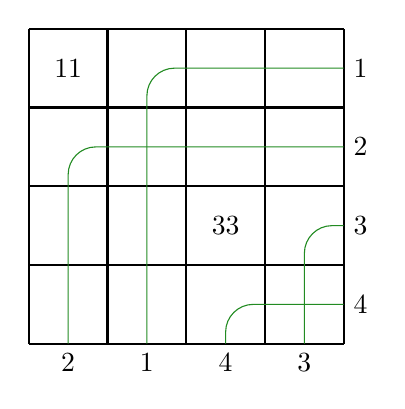
\begin{tikzpicture}
    \draw [step=1.0, thick] (0,0) grid (4,4);
    \draw [rounded corners=10pt, ForestGreen] (0.5,0) node [below, black] {$2$} -- (0.5,2.5) -- (4,2.5) node [right, black] {$2$};
    \draw [rounded corners=10pt, ForestGreen] (1.5,0) node [below, black] {$1$} -- (1.5,3.5) -- (4,3.5) node [right, black] {$1$};
    \draw [rounded corners=10pt, ForestGreen] (2.5,0) node [below, black] {$4$} -- (2.5,0.5) -- (4,0.5) node [right, black] {$4$};
    \draw [rounded corners=10pt, ForestGreen] (3.5,0) node [below, black] {$3$} -- (3.5,1.5) -- (4,1.5) node [right, black] {$3$};
    \draw node at (0.5, 3.5) {$11$};
    \draw node at (2.5, 1.5) {$33$};
\end{tikzpicture}
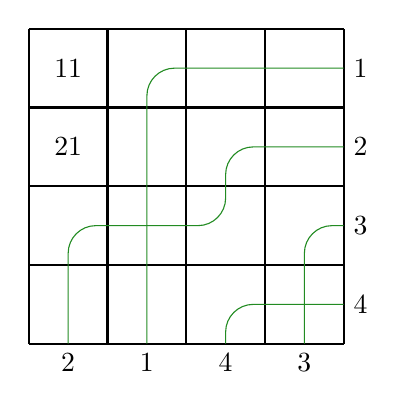
\begin{tikzpicture}
    \draw [step=1.0, thick] (0,0) grid (4,4);
    \draw [rounded corners=10pt, ForestGreen] (0.5,0) node [below, black] {$2$} -- (0.5,1.5) -- (2.5,1.5) -- (2.5, 2.5) -- (4,2.5) node [right, black] {$2$};
    \draw [rounded corners=10pt, ForestGreen] (1.5,0) node [below, black] {$1$} -- (1.5,3.5) -- (4,3.5) node [right, black] {$1$};
    \draw [rounded corners=10pt, ForestGreen] (2.5,0) node [below, black] {$4$} -- (2.5,0.5) -- (4,0.5) node [right, black] {$4$};
    \draw [rounded corners=10pt, ForestGreen] (3.5,0) node [below, black] {$3$} -- (3.5,1.5) -- (4,1.5) node [right, black] {$3$};
    \draw node at (0.5, 3.5) {$11$};
    \draw node at (0.5, 2.5) {$21$};
\end{tikzpicture}
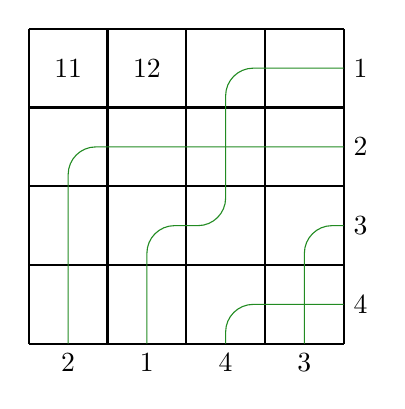
\begin{tikzpicture}
    \draw [step=1.0, thick] (0,0) grid (4,4);
    \draw [rounded corners=10pt, ForestGreen] (0.5,0) node [below, black] {$2$} -- (0.5,2.5) -- (4,2.5) node [right, black] {$2$};
    \draw [rounded corners=10pt, ForestGreen] (1.5,0) node [below, black] {$1$} -- (1.5,1.5) -- (2.5, 1.5) -- (2.5, 3.5) -- (4,3.5) node [right, black] {$1$};
    \draw [rounded corners=10pt, ForestGreen] (2.5,0) node [below, black] {$4$} -- (2.5,0.5) -- (4,0.5) node [right, black] {$4$};
    \draw [rounded corners=10pt, ForestGreen] (3.5,0) node [below, black] {$3$} -- (3.5,1.5) -- (4,1.5) node [right, black] {$3$};
    \draw node at (0.5, 3.5) {$11$};
    \draw node at (1.5, 3.5) {$12$};
\end{tikzpicture}
\end{center}
Notice that (this appeals to the example that i havent done yet)
\begin{align*}
    in_{diag} &= (z_{11},  z_{33} z_{21} z_{12})\\
    &= (z_{11} ,  z_{33}) \cap ( z_{11} ,  z_{21}) \cap ( z_{11} ,  z_{12})
\end{align*}
and the correspondence between the empty spaces in the BPDs and the ideals.
\end{example}


\begin{theorem}
    For many diagonal orders, the radical of the initial ideal 
    \begin{align*}
        \sqrt{ in_{diag} (I_\omega) } = \bigcap_{P \in BPD(\omega} (z_{ij} \mid P \text{ has empty square in position } (i,j) ).
    \end{align*}
    Moreover, the degree of a component equals the number of BPDs with an empty square in those positions.
\end{theorem}

\begin{example}
    For $\omega = 321654$ there are exactly two BPDs with the top left $6$ boxes empty, and so one component has degree $2$.
\end{example}

\begin{remark}
    Some questions we still have:
    \begin{itemize}
        \item When is $in_{diag} (I_\omega ) $ radical?\\
        - Probably pattern avoidance.
        \item When are there embedded components?\\
        - Possibly only when top degree fuzz but who knows.
    \end{itemize}
\end{remark}

We have reached the state of the art for this family of determinental varieties, now we will move to related topics.

\subsection{Skew-Symmetric Matrices}

We can consider skew-symmetric matrices (SSM) with similar NW rank conditions:

\begin{align*}
    \set{ X \in Mat_{n \times n} \mid X^t = - X \text{ and } rank (X_{[i], [j]} ) \leq r(i,j)  }.
\end{align*}

We require the diagonals to be all zero to deal with the $char( F) = 2$ edge case. The irreducibles are indexed by fixed point free involutions, eg $\omega \in S_n $ such that $\omega ( \omega (i) ) = i \neq \omega (i) $ for all $i$.

\begin{theorem}
    We have that
    \begin{itemize}
        \item The defining determinants don't generate a radical ideal. The radical is generated by a set of ``Pfaffians" (square of determinants).
        \item There is a more complicated set of Pfaffians that is a GB for the radical with respect to a particular antidiagonal order.
        \item For this term order, the initial ideal is square-free and CM (as it is vertex-decomposable, which implies our original space is CM).
    \end{itemize}
    For this term order, the prime decomposition of the initial ideal is governed by ``fpf involution pipe dreams".
\end{theorem}

\begin{remark}
    Some questions:
    \begin{itemize}
        \item What about other orders?
        \item What about regularity?\\
        - St Denis has some results in some cases.
        \item What about SSM with SW rank conditions?\\
        - This is super hard.
        \item What about symmetric matrices with NW rank conditions?\\
        - These aren't CM ($351624$)! These aren't ``normal" either (ie super bad).
        - What about symmetric matrices with SW rank justification?
    \end{itemize}
\end{remark}

\begin{theorem}
    For symmetric matrices with SW rank conditions, the defining equations are a diagonal Grobner basis.
\end{theorem}

\begin{remark}
    The diagonal initial ideal is square-free.
\end{remark}

\begin{theorem}
    CM since diagonal, $in_{ideal} $ is Stanley-Reisner ideal of a type C subword complex.
\end{theorem}

\begin{remark}
    The facets here are given by type C pipe dreams. What about regularity?
\end{remark}

\begin{definition}
    Double determinental varieties are
    \begin{align*}
        D_{m,n,r,s,t} = \set{ (X_1 , \cdots, X_r) \in Mat_{m \times n}^r \mid rank ( X_1 \mid \cdots \mid X_r) \leq s, rank \left( \begin{smallmatrix} X_1 \\ \vdots \\ X_r \end{smallmatrix} \leq t \right)}.
    \end{align*}
\end{definition}

\begin{theorem}
    The defining equations of $D_{m,n,r,s,t}$ generate a prime ideal. The defining equations are a GB under any (anti)diagonal term order. The initial ideal is a Stanley-Reisner ideal of a vertex decomposable simplical complex, so both ideals are CM.
\end{theorem}

\begin{definition}
    Let $G$ be a simple graph on $[n]$. Let 
    \begin{align*}
        I_G = ( x_i x_j \mid ij \in E(G)) \subset K[x_1, \cdots , x_n]
    \end{align*}
    be the edge ideal of $G$.
\end{definition}

\begin{proposition}
    We have that
    \begin{align*}
        \dim ( S/ I_G) = \alpha (G).
    \end{align*}
\end{proposition}

\begin{definition}
    Let
    \begin{align*}
        reg'(S / I_G) = deg (K((S / I_G)) - codim (S/ I_G).
    \end{align*}
\end{definition}

\begin{theorem}
    For any $r,r' \geq 1$, there is a monomial ideal $I$ with $reg (S/I) = r$ and $reg' (S/I) = r'$.
\end{theorem}

\begin{theorem}
    In previous theorem, we can restrict to edge ideals and the result still holds. However if $\abs{V(G)} = n$ then $reg + reg' \leq n$.
\end{theorem}

\begin{remark}
    Some questions:
    \begin{itemize}
        \item Fix $\abs{V(G) } = n$. What pairs $(reg, reg')$ can occur? Is it the integer points of a convex lattice polygon?
        \item Fix $n,r,r'$. What percentage of $n$-vertex graph ideals have $reg = r, reg' = r'$?
    \end{itemize}
\end{remark}